%-------------------------------------------------------------------------------
% Preamble
%-------------------------------------------------------------------------------

\documentclass[a4paper, 12pt]{article}
\usepackage{ms}            % load the template
\usepackage[osf]{mathpazo} % palatino
%\usepackage[round]{natbib} % author-year citations
\usepackage[superscript,biblabel]{cite} % for superscript citations
\usepackage{graphicx}
\usepackage{subcaption}
\usepackage{parskip} 
\usepackage{amsmath}
\usepackage{longtable}
\usepackage{pdflscape}

\pagenumbering{arabic}  
\linespread{1.66}

%-------------------------------------------------------------------------------
% Title page information
%-------------------------------------------------------------------------------

\title{Clade-wide variation in bite-force performance is determined primarily by size not ecology.}
\author{}
\date{}
\affiliation{}

\author{
 Justin E Isip$^{1,2*}$,
 Natalie Cooper$^{1}$, 
 Marc EH Jones$^{3}$, 
}
 \date{}
\affiliation{\noindent{\footnotesize
  $^1$Department of Life Sciences, Natural History Museum London, Cromwell Road, London, SW7 5BD, UK.\\
  $^2$Department of Life Sciences (Silwood Park), Imperial College London, Ascot, UK.\\ 
  $^3$Research Department of Cell and Developmental Biology, Anatomy Building, University College London, Gower Street, London, WCIE 6BT, UK.\\
  $*$Email address: justin.isip.21@ucl.ac.uk 
}}

\vfill

\runninghead{Bite-force variation}

%-------------------------------------------------------------------------------
% Begin document
%-------------------------------------------------------------------------------
\begin{document}
\modulolinenumbers[1]   % Line numbering on every line

\mstitlepage

\parindent = 1.5em
\addtolength{\parskip}{.9em}

\raggedright

\newpage

%-------------------------------------------------------------------------------
% Abstract
%-------------------------------------------------------------------------------

\section{Abstract}

Performance traits are tightly linked to the fitness of organisms. 
However, because studies of variation in performance traits generally focus on just one or several closely-related species, we are unable to draw broader conclusions about how and why these traits vary across clades. 
One important performance trait related to many aspects of an animal's life history is bite-force.  
Here we use a clade-wide phylogenetic comparative approach to investigate relationships between size, head dimensions and bite-force among lizards and tuatara (lepidosaurs), using the largest bite-force dataset collated to date for any taxonomic group. 
We test four predictions: that bite-force will be greater in larger species, and for a given body size, bite-force will be greatest in species with acrodont tooth attachment, herbivorous diets, and non-burrowing habits. 
We show that bite-force is strongly related to body and head size across lepidosaurs and, as predicted, larger species have the greatest bite-forces. 
Contrary to our other predictions, tooth attachment, diet and habit have little predictive power when accounting for size. Herbivores bite more forcefully simply because they are larger. 
Our results also highlight priorities for future sampling to further enhance our understanding of broader evolutionary patterns.

\textbf{Keywords: biteforce, diet, lizard, tuatara, Lepidosauria}

%-------------------------------------------------------------------------------
% Main text
%-------------------------------------------------------------------------------

\section{Introduction}

Performance traits are of vital importance for activities that influence organism survival, such as food acquisition, predator avoidance, and mate acquisition\cite{lailvaux2004performance,legalliard2004,lappin2005weapon,irschick2008}. 
Due to the direct links between performance and fitness, we expect these traits to be under strong selection\cite{arnold1983,irschick2008} however, relatively few studies of natural selection in the wild have focused on performance traits\cite{irschick2008,kingsolver2012} and, due to limited time and resources, most studies focus on just one or several species, limiting our ability to draw broader conclusions about how and why performance traits vary across clades\cite{irschick2008}. 
Bite-force is an important performance trait with close ties to ecology and life history\cite{herrel1999morphology,anderson2008bite,erickson2014comparative,lappin2014reliable,husak2009fitness}. 
Greater bite-force may reduce prey handling times and increase dietary breadth\cite{herrel1999morphology,herrel2004omnivory,verwaijen2002relationships,van2006seed,taverne2020proximate}, can increase the likelihood of success in territory defence and male-male combat\cite{lailvaux2004performance,lappin2005weapon,huyghe2005morphology,husak2006bite}, and boost reproductive success\cite{lappin2005weapon,husak2006bite,husak2009fitness}.
Crucially, bite force data are relatively simple to collect; voluntary \textit{in vivo} bite-force has been successfully measured in a wide range of taxa, including sharks, frogs, lizards, crocodylians, rodents, and bats(e.g. \cite{herrel1999morphology,huber2005analysis,santana2010mechanics,becerra2013biting,erickson2014comparative,lappin2014reliable,lappin2017bite}). 
To date, however, large scale analyses of variation in bite-force and its relationship to key traits such as diet, body size, and habit are lacking. 
Most bite force studies instead focus on a single species (e.g.\cite{husak2006bite}) or a set of closely related species (e.g.\cite{taverne2020proximate}).
A clade-wide comparative approach is required to understand how and why bite-force varies among species and to test related hypotheses.

In this study we use a clade-wide comparative approach to investigate variation in bite-force within lizards and tuatara (i.e. Lepidosauria minus Serpentes for which very little bite force data exists) in relation to species' morphological and ecological traits. 
We use lepidosaurs because most studies of bite force have focused on these species due to their experimental tractability and the key importance of bite-force to many aspects of their ecology and life history\cite{herrel1999morphology,lappin2014reliable}.
Lepidosaurs are also an ideal group on which to test many hypotheses about variation in bite force because they are diverse in terms of species richness (7,262 species\cite{uetz2020reptile}), diet\cite{cooper2002distribution}, food processing\cite{mcbrayer2002prey}, life habit\cite{meiri2018traits}, muscle anatomy \cite{haas1973muscles,daza2011jaw}, tooth attachment\cite{jenkins2020bite}, and skull shape\cite{metzger2005correlations}. 
Here we test the following predictions about variation in bite-force within lizards and tuatara using the largest dataset of existing \textit{in vivo} bite-force data collated to date, and phylogenetic generalised least squares (PGLS) analyses.

\begin{enumerate}

\item \textit{Larger species, in terms of body and head size, will have greater bite forces.} 
Bite-force tends to show positive allometric scaling with morphological traits, as larger individuals will have more muscle mass and presumably a greater bite-force \cite{aguirre2002ecomorphological,herrel2004omnivory,lailvaux2004performance,vanhooydonck2005does,MEASEY2009217}, but this has not been tested across a broad taxonomic group. 
Independent of differences in overall body size, head dimensions are also strongly associated with bite-force performance\cite{kaliontzopoulou2012relationships,jones2020reproductive}, as animals with larger or wider heads are assumed to accommodate more jaw musculature which results in a greater bite-force\cite{herrel1999morphology,huyghe2005morphology}.

\item \textit{Species with acrodont tooth implantation will have greater bite force than those with non-acrodont tooth implantation for a given size.} 
Acrodonty, where the teeth attach to the crest of the jaw bone rather than elsewhere \cite{smith1958evolutionary}, has long been associated with greater anchorage and greater loading (e.g.\cite{smith1958evolutionary,jones2008skull}) and recent analyses appear to support that association \cite{jenkins2020bite}.
However, an analysis accounting for phylogeny has yet to be attempted.

\item \textit{Herbivorous species will have the greatest bite forces for a given size.}
Herbivorous species are often considered to have greater bite-forces than carnivores and omnivores due to the forces required to process fibrous plant material\cite{cooper2002distribution,herrel1999morphology,metzger2005correlations,herrel2004omnivory,Herrel2008}.
However, a relationship between bite force and diet across lepidosaurs more broadly has never been tested, and some studies suggest carnivores, especially species that feed upon hard-shelled prey (e.g. shelled molluscs, crabs, corals etc.), may exhibit greater maximum bite-forces (e.g.\cite{schaerlaeken2012built}).

\item \textit{Burrowing species will have lower bite forces than non-burrowing species of a given size.}
Bite force may also vary with substrate (or life habit) due to selection pressures and constraints imposed on feeding apparatus such as the skull structure (e.g.\cite{gray2019evolution}).
Burrowing can restrict head width\cite{vanhooydonck2011push} and may, in turn, restrict relative jaw muscle volume. We predict that these constraints will result in lower bite forces in burrowing species. 

\end{enumerate}

%-------------------------------------------------------------------------------
% Methods
%-------------------------------------------------------------------------------

\section{Materials and Methods}

\subsection{Data collection}

\subsubsection{Bite force and morphological data}
We surveyed all studies published between 1999 (when the first in vivo bite-force data were collected for lizards) and 2020, reporting empirical data on \textit{in vivo} bite-force performance in lizards and tuatara, using the VolBif bite-force database \cite{lappin2014reliable} supplemented with Google Scholar searches with search terms: bite, force, performance, transducer, and Kistler. 
We excluded studies where the bite-force and morphological data came from different animals, where only residual or size corrected bite-force data were provided, or where bite-force was provided without body size data. 
These requirements left us with 53 published studies (out of 111) that had bite-force data for one or more species, comprising 164 species in total. 

We collated mean maximum bite force $\pm$ standard error (N) from each of the 53 studies with appropriate data, for each species within the publication, and for females and males separately where possible. 
We used bite forces extracted from the tips of the jaw rather than the posterior end of the jaw where specified\cite{lappin2014reliable}, and when there was more than one population with bite-force data available for a species within a publication, we used the population with the greatest bite-force. 
For each bite force record we recorded the (1) species name; (2) sex; (3) age (adult or juvenile); (4) sample size for bite-force data; (5) snout-vent length (SVL; mm); (6) head width (mm); (7) head length (mm); (8) head height (mm); and (9) sample size for morphometric data. 
For the morphological measurements we collected the mean $\pm$ standard error values. 

\subsubsection{Ecological and phylogenetic data}

For prediction 2, all Acrodonta and the tuatara were classified as acrodont and the rest of the species were classified as non-acrodont.
Trogonophidae are sometimes classified as acrodont\cite{jenkins2020bite}, so we repeated the analyses with this family in the acrodont category.
We used diet and substrate data provided in ref\cite{meiri2018traits}, with additional data from ref\cite{metzger2005correlations} and ref\cite{cooper2002distribution}. 
Diets were classified as carnivorous, herbivorous, or omnivorous based on whether animals, plants or both made up the greatest proportion of the diet (prediction 3\cite{meiri2018traits}).
Three species (\textit{Anolis singularis}, \textit{Pygomeles braconnieri} and \textit{Scelotes montispectus}) had no diet data and were excluded from the diet analyses. 
The substrate/life habit data\cite{meiri2018traits} consisted of 14 different categories, so we created a fossorial variable (Fossorial versus all other categories) to test prediction 4.  
We also explored whether saxicolous (crevice dwelling) or arboreal species had significantly different bite-forces for their size using two new variables: arboreal (Arboreal versus all other categories), and saxicolous (Arboreal/Saxicolous, Arboreal/Terrestrial/Saxicolous, Saxicolous, Terrestrial/Saxicolous versus all other categories). 
We also investigated differences across clades, using the classification of Burbrink \textit{et al.}\cite{burbrink2020interrogating} to define eight more inclusive clades (Acrodonta, Anguimorpha, Dibamia, Gekkota, Lacertoidea, Pleurodonta, Rhynchocephalia and Scincoidea). 

For the phylogenetic generalised least squares (PGLS) analyses (see below) we used the dated molecular phylogeny of Wright \textit{et al.}\cite{wright2015came} and pruned it to the species in our dataset. 
Eight species were in our dataset but missing from the tree. We added five of these species to the tree using information from other published phylogenies to determine where they fitted into the tree (Table S1) and an arbitrary branch length of 0.1. 
Note that we repeated all analyses using only the species in the original tree to ensure this procedure did not bias our results. We were unable to find data on the phylogenetic relationships of three species (\textit{Aspidoscelis sonorae}, \textit{Diplolaemus leopardinus} and \textit{Tropidurus semitaeniatus}) leaving 161 species in the phylogeny.

\subsubsection{Data cleaning and processing}
Prior to analyses we cleaned the data using the tidyverse package \cite{wickham2019welcome} in R \cite{R-Core-Team:2020}. 
We removed juveniles and sub-adults from the dataset and corrected species binomial names and family names using The Reptile Database \cite{uetz2020reptile}. 

Maximum values are the most appropriate measure for comparing performance \cite{hertz1988time,losos2002cautionary}. 
For each species, we therefore selected the study with the highest maximum bite-force. 
If two or more studies of the same species had the same maximum bite-force value, we used the study with the most complete data for the other variables. 
Note that we used the morphological data associated with the study that had the maximum bite-force for each species to ensure these data came from the same animals. 
Finally we also created datasets that included only females or only males. 
All raw and cleaned data are available on the NHM Data Portal (https://doi.org/10.5519/dkrhpxjh\cite{lepidosaurdata}). 

\subsection{Analyses}
All statistical analyses used R version 4.0 \cite{R-Core-Team:2020} and reproducible R scripts are available on GitHub ( https://github.com/nhcooper123/lepidosaur-biteforce). 
All continuous variables were natural log-transformed prior to analyses. 
Results were visualised using ggtree \cite{yu2017ggtree} and ggplot2 \cite{wickham2011ggplot2}.

\subsubsection{Dataset coverage}
We calculated the total numbers and percentage coverage of all 164 species in our dataset from each family recognised in Uetz \textit{et al.}\cite{uetz2020reptile} and clade\cite{burbrink2020interrogating}, and for lizards and tuatara as a whole.
We explored the distribution of raw bite-force (i.e. bite-force values before correcting for size differences) across clades and families, and within tooth attachment, diet and substrate categories, and visualised the differences in bite-force and the four size measures in the full dataset, and the data for females and males separately.

\subsubsection{Predicted correlates of bite-force}
We used phylogenetic generalised least squares (PGLS) models (with maximum likelihood estimates of Pagel’s $\lambda$) to test our predictions.
PGLS models account for the non-independence of trait values in close relatives by incorporating information about phylogenetic relationships into the error term of the model. 
This approach deals with the problem of phylogenetic pseudoreplication \cite{harvey1991comparative}. 
We fitted PGLS models using the R package caper \cite{orme2018caper}, and performed standard model checks for GLS models (Q-Q plot, histogram of residuals, residuals versus linear predictors, response versus fitted values) to assess model fit. 

First we used PGLS models to investigate the relationship between maximum bite-force and size, using SVL ($n = 161$), head width ($n = 142$), head height ($n = 136$), or head length ($n = 136$), to represent size (prediction 1). 
Next we fitted PGLS models testing whether the relationship between maximum bite-force and size (SVL, head width, head height, or head length) varied with (i) tooth attachment (prediction 2); (ii) diet (prediction 3);  (iv) whether species were purely fossorial or not (prediction 4).
We additionally tested whether the relationship between maximum bite-force and size varied with clade, whether species were purely arboreal or not, and whether species were saxicolous or not. 
For the clade analyses we excluded Anguimorpha, Gekkota and Rhynchocephalia because they had fewer than 10 species in the dataset, and for females and males separately we also excluded Scincoidea because we had only one sexed skink species. 
Finally, we Bonferroni corrected our p-values to account for multiple comparisons.

In many species of lizards, males have larger heads than females and thus we expect some sexual dimorphism in bite-force \cite{herrel1999sexual,verwaijen2002relationships}. 
We initially used data from both sexes combined, but repeated each analysis using just females, and just males (except for the fossoriality analyses where only one fossorial species had known sex). 
We also ran each analysis using the original 156 species tree without the five added taxa to ensure this difference in sampling did not bias our results. 

%-------------------------------------------------------------------------------
% Results
%-------------------------------------------------------------------------------

\section{Results}

\subsubsection{Dataset coverage}
The final cleaned dataset contained bite-force data for 164 species overall, 112 species when only data from females were used and 132 when only data from males were used. 
Body size (SVL) ranged from 31.62 mm to 425 mm.
 

Overall, our dataset included only 2.26\% of 7,262 extant lizard and tuatara species\cite{uetz2020reptile}, and these were extremely skewed phylogenetically and taxonomically (Figure \ref{fig-data-coverage}, Figure S1, Tables S2-3). 
Over 45\% of our species sample (74 species) are members of Pleurodonta. 
However, these 74 species represent only $~6$\% of the diversity of Pleurodonta. 
No family had more than 25\% species coverage, except Sphenodontidae which contains only one extant species and had 100\% coverage (Figure \ref{fig-data-coverage}, Table S2). 
24 of the 44 families (54.5\%; Figure \ref{fig-data-coverage}, Table S2), and one clade (Dibamia; Figure S1, Table S3) had no species with bite-force data we could use in this study. 

Raw bite-force, i.e. bite-force values before correcting for size differences, ranged from 0.12 N to 534.24 N, and varied among clades, families, and within tooth attachment, diet, and substrate categories (Figures S2-S3; Table S4). 
Overall, females have lower bite-forces and slightly smaller body and head dimensions than males (Figure S4).

\subsubsection{Predicted correlates of bite-force}
We were unable to place three species (\textit{Aspidoscelis sonorae}, \textit{Diplolaemus leopardinus} and \textit{Tropidurus semitaeniatus}) within the phylogeny, meaning that the analyses used only 161 species. 
Each analysis contained slightly different numbers of species (due to the three species without diet data, the 19 species without head width data and the 25 species without head length or head height data).

All analyses of all subsets of the data show strong, significant, positive correlations among bite-force and all measures of size (prediction 1; Figure 2; Tables S5-S6). 
The large negative outliers on the plots showing the relationship between bite-force and SVL are skinks (Scincoidea; Figure \ref{fig-size-biteforce}A). 
The skinks in our dataset have long bodies relative to their head size in comparison with other lizards. 
This difference in body shape results in some skinks appearing to have much lower bite-force than other groups given their SVL, but this effect disappears if we use head dimensions as proxies for size instead (Figure \ref{fig-size-biteforce}B-D).

The relationship between bite-force and size did not vary significantly with tooth attachment (prediction 2), for all four measures of size (Table 1; Figure S5), for the full dataset and for females and males separately (Tables S7-S8). 
The results were qualitatively similar when Trogonophidae were categorised as acrodont (Table S9).


The relationship between bite-force and size varied significantly with diet (prediction 3), but only when using head width as the measure of size for the full dataset (Table 1; Figure \ref{fig-diet}), and head width or head length using only females (Tables S7-S8). 
This result reflects a very small, but significant difference between the intercepts of carnivores and omnivores. 
Herbivores did not differ significantly from carnivores or omnivores, but were larger on average than the other two dietary groups (Figure S6; mean SVL herbivores = 192.8 mm; mean SVL of non-herbivores = 86.85 mm).

There was a significant effect of fossoriality on the relationship between bite-force and size for all size measures except SVL (prediction 4; Table 1; Figure \ref{fig-fossorial}). 
Fossorial species had higher bite-forces for their head dimensions compared to non-fossorial species, though the slope of the relationship was not significantly different (Table 1; Figure \ref{fig-fossorial}). 
Note that because only one fossorial species was sexed we were unable to run separate models for females and males. 

The relationship between bite-force and size did not vary significantly with clade, whether species were purely arboreal or not or whether species were saxicolous or not. 
This was the case using all four measures of size (Table S10; Figure \ref{fig-size-biteforce}, Figures S7-S8), for the full dataset and for females and males separately (Tables S7-S8). 

Results using the original 156 species tree are in the Supplementary Materials (Tables S6 and S11) but were qualitatively identical to those using the full 161 species tree.

%-------------------------------------------------------------------------------
% Discussion
%-------------------------------------------------------------------------------

\section{Discussion}

Bite-force was strongly positively correlated with snout-vent length and head dimensions across the 161 species in our analyses. 
This relationship varied with some aspects of species ecology; for certain head measurements carnivorous species had greater bite-forces compared to omnivores, and fossorial species had higher bite-forces for their head dimensions compared to non-fossorial species. 
There was no significant variation with clade, tooth attachment, or whether species were purely arboreal or not, or saxicolous or not. 
These results support some of our predictions, but not all, as discussed below.

Despite the great variety of morphologies and ecologies represented by the lepidosaurs in our sample, size always appeared to be the most important variable in explaining variation among species. 
The strong correlations among size measures and bite-force matches that found in mammals, turtles, and crocodylians e.g.\cite{aguirre2002ecomorphological,marshall2012ontogenetic,becerra2013biting,erickson2014comparative}.
This pattern also parallels results from other lepidosaur studies of narrower taxonomic breadth \cite{lailvaux2004performance,vanhooydonck2005does,MEASEY2009217,jones2020reproductive}.
The only group for which this pattern was less clear was Scincoidea. 
However, many skinks have long bodies in relation to their head size (e.g.\cite{wiens2006does}), meaning their bite-force was lower than expected in relation to their snout-vent length, but scaled more similarly to other taxonomic groups for their head dimensions. 
The close relationship between bite-force and size is almost certainly due to the close relationship between size and jaw muscle cross-sectional area. 
Muscles with greater cross-sectional area are generally able to generate greater force \cite{groning2013importance,sellers2017ontogeny}, thus providing more forceful bites. 
Large animals are usually able to bite more forcefully than smaller animals regardless of other factors such as head shape or diet. 

We did not find support for our second prediction, that species with acrodont tooth implantation would have greater bite force than those with non-acrodont tooth implantation. 
There are several lizards with forceful bites that are not acrodont which may explain this result. 
In addition, our two tooth attachment categories may not adequately represent the range of tooth implantation anatomy in extant Lepidosauria. Non-acrodonty encompases a range of variation that includes teeth with deep lingual roots and minimal alveolar bone and teeth with shallow lingual roots and extensive alveolar bone\cite{smith1958evolutionary,presch1974,berkovitz2017}. 
Given the spectrum of variation known in tooth attachment in lepidosaurs\cite{bertin2018current}, and that tooth implantation can also vary along the tooth in some taxa, tooth attachment may be related to the direction (compression and tension) and magnitude of local loading conditions during biting behaviour rather than overall bite force capacity \textit{per se}. 
 
Our results also do not support our third prediction, that herbivorous species would have the greatest bite forces.
Previous studies have suggested that herbivorous lepidosaurs have greater bite-forces, on average, than carnivores or omnivores due to their larger jaw muscles for processing plant material \cite{metzger2005correlations,cooper2002distribution,herrel1999morphology,herrel1999sexual,herrel2004omnivory,Herrel2008,herrel2014does}.
These suggestions were based on comparisons among a few species e.g.\cite{herrel2014does,herrel2004omnivory} or within a genus e.g.\cite{lopez2015sex}, so our taxonomic sample is much broader here and highlights the benefit of a clade-wide comparative approach. 
Our results confirm that herbivores did tend to have greater bite-forces, but this result reflects the fact that herbivores were larger on average, in both snout-vent length and head dimensions, than their carnivorous or omnivorous counterparts, and size was the strongest predictor of bite-force. 
Plant consumption in lepidosaurs has been linked to increased size \cite{cooper2002distribution,herrel2014does,metzger2005correlations}, perhaps because of the lower mass-specific metabolic requirements of larger individuals, or the increased space for the digestive system allowing more efficient digestion of tough plant material in larger individuals\cite{herrel2014does,espinoza2004recurrent}.
Our results, however, showed that herbivores did not have significantly greater bite-forces than expected given their size. This result suggests that herbivores tend to bite more forcefully merely because they are larger, not because of any specialised adaptations for herbivory. 

Finally our fourth prediction was also not supported by our results; in fact fossorial species bite more forcefully than expected given their head dimensions.
Previous studies have suggested a trade-off between burrowing and bite-force: greater head width accommodates larger jaw muscles but also increases the cross-sectional area that must displace burrowing medium (e.g. soil, sand, plant matter). 
In the fossorial skink \textit{Acontias percivali}, narrow-headed individuals were able to dig into the substrate much faster than broader-headed individuals, but bite-force was greater in individuals with relatively wider heads\cite{vanhooydonck2011push} (although see\cite{le2020trade}).
Similarly, in the amphisbaenid \textit{Leposternon microcephalum}, the energetic costs associated with burrowing increase exponentially with body and head size\cite{navas2004morphological}.
Our results suggest that, at least for the species in our dataset, fossorial lepidosaurs are able to overcome this trade-off and bite more forcefully than their head dimension alone would predict. 
This result may suggest that fossorial species require greater bite force than non-fossorial lizards whether it be due to the range of prey that they encounter or the importance of biting when gape is limited (and thus swallowing prey whole is not possible) . 
However, 11 of the 12 fossorial species available to our analyses were skinks (the remaining species is the amphisbaenian \textit{Trogonophis wiegmanni}).
Therefore, the result may reflect differences particular to Scincoidea rather than burrowing lepidosaurs in general.
There are no obvious differences in jaw mechanism or jaw muscle arrangement known for Scincoidea that might increase bite-force capacity (e.g.\cite{haas1973muscles,daza2011jaw}), but future studies should pay greater attention to details of jaw muscle pennation structure. 
Alternatively skinks may be particularly aggressive and/or cooperative for bite-force data collection, or perhaps bite-force was collected in a slightly different manner for these 11 species. 
Data from additional non-fossorial scincoids or other fossorial lepidosaurs should help address this issue.
The longer bodies relative to head size in skinks also explains why we did not find a significant effect of fossoriality on the relationship between snout-vent length and bite-force because, as described above, skinks have a lower bite-force than expected given their snout-vent length. 

Although there have been over 100 studies of bite-force on lizards and tuatara, many species remain unexamined. 
Some of these species are either too small (e.g. \textit{Brookesia} sp.) or are uncooperative (e.g. \textit{Ophisaurus} sp.; MEHJ \textit{pers. obs.}). 
Our dataset encompassed only 2.26\% of the 7,262 existing lizard and tuatara species\cite{uetz2020reptile}, and this sample was heavily skewed towards certain clades and ecologies. 
Despite including an order of magnitude more species than previous studies, we still had no data from any species within Dibamia or within 24 lizard families, and only had data for 11 herbivores. 
Small herbivores (for example various species within Leiolaemidae; average SVL $< 100 mm$\cite{espinoza2004recurrent}) are conspicuously missing from the bite-force literature. 
Additionally, our dataset was limited not only by the number of species that have been investigated for bite-force, but by the availability of these data in the literature. Of the 111 published studies we collated, less than half (n = 53) contained openly accessible/usable data. 
This issue prevents larger comparative studies being undertaken. 
Future studies should provide their raw individual bite-force and morphological measurement data to enable future studies to build on previous work. 
This study represents the first rigorous step in examining bite-force across an entire clade while accounting for phylogenetic relationships among species, providing a framework for future work. 

%-------------------------------------------------------------------------------
% Additional stuff
%-------------------------------------------------------------------------------

\section{Acknowledgments}
We thank previous authors for sharing their data. We thank  St\'ephane J. Montuelle and Geoff While for correspondence, Kris Lappin and Mark Hutchinson for discussion, and Roger Seymour for feedback on an earlier version of this manuscript.

\section{Data accessibility}
Data are available from the NHM Data Portal (https://doi.org/10.5519/dkrhpxjh\cite{lepidosaurdata}). 
R code is available from GitHub (https://github.com/nhcooper123/lepidosaur-biteforce; Zenodo DOI: to add on acceptance).

%-------------------------------------------------------------------------------
% References
%-------------------------------------------------------------------------------

\bibliographystyle{bibstyle}
\bibliography{biteforce}

%-------------------------------------------------------------------------------
% Tables
%-------------------------------------------------------------------------------
\newpage
%\section{Tables}

\begin{landscape}
  % Table 1

\begin{longtable}{lccccccccccccccc}

\caption{Results from phylogenetic generalised least squares (PGLS) models of bite-force as a function of size, one of three covariates (tooth attachment type, diet, fossorial or not) and their interaction term. Size was snout vent length (SVL; mm), head width (HW; mm), head length (HL; mm), or head height (HH; mm). Significant p values are highlighted in bold. Bonferroni corrected p values (bonf p) are provided for all terms except the size term for which Bonferroni corrected p values were always $<$ 0.001. res df = residual degrees of freedom. df = degrees of freedom. $\lambda$ = Pagel's $\lambda$.}\\ 


% Header 1
\hline

\multicolumn{5}{c}{} &
\multicolumn{3}{c}{\textbf{size}} &
\multicolumn{4}{c}{\textbf{covariate}} &
\multicolumn{4}{c}{\textbf{interaction}}\\

  % Header 2
  \hline
  \textbf{covariate} &
  \textbf{size} &
  \textbf{res df} &
  \textbf{$\lambda$} &
  \textbf{r$^2$} &
  \textbf{df} &
  \textbf{F} &
  \textbf{p} &
  \textbf{df} &
  \textbf{F} &
  \textbf{p} &
  \textbf{bonf p} &
  \textbf{df} &
  \textbf{F} &
  \textbf{p} &
  \textbf{bonf p} \\

  % Body of table
\hline
tooth attachment & SVL & 157 & 0.946 & 0.723 & 1.000 & 416.8 & \textbf{$<$ 0.001} & 1.000 & 0.767 & 0.382 & 1.000 & 1.000 & 3.187 & 0.076 & 1.000 \\ 
tooth attachment & HW & 138 & 0.982 & 0.741 & 1.000 & 403.6 & \textbf{$<$ 0.001} & 1.000 & 0.053 & 0.818 & 1.000 & 1.000 & 3.049 & 0.083 & 1.000 \\ 
tooth attachment & HL & 132 & 0.96 & 0.709 & 1.000 & 330.1 & \textbf{$<$ 0.001} & 1.000 & 0.764 & 0.384 & 1.000 & 1.000 & 1.270 & 0.262 & 1.000 \\ 
tooth attachment & HH & 132 & 0.703 & 0.822 & 1.000 & 622.9 & \textbf{$<$ 0.001} & 1.000 & 0.344 & 0.558 & 1.000 & 1.000 & 1.230 & 0.269 & 1.000 \\ 
diet & SVL & 152 & 0.953 & 0.714 & 1.000 & 393.4 & \textbf{$<$ 0.001} & 2.000 & 0.706 & 0.495 & 1.000 & 2.000 & 1.008 & 0.367 & 1.000 \\ 
diet & HW & 133 & 1.000 & 0.806 & 1.000 & 546.8 & \textbf{$<$ 0.001} & 2.000 & 13.75 & \textbf{$<$ 0.001} & \textbf{$<$ 0.001} & 2.000 & 1.150 & 0.320 & 1.000 \\ 
diet & HL & 127 & 0.967 & 0.704 & 1.000 & 316.9 & \textbf{$<$ 0.001} & 2.000 & 1.026 & 0.362 & 1.000 & 2.000 & 0.328 & 0.721 & 1.000 \\ 
diet & HH & 127 & 0.681 & 0.822 & 1.000 & 613.5 & \textbf{$<$ 0.001} & 2.000 & 0.900 & 0.409 & 1.000 & 2.000 & 0.603 & 0.549 & 1.000 \\ 
fossorial & SVL & 157 & 0.949 & 0.741 & 1.000 & 445.3 & \textbf{$<$ 0.001} & 1.000 & 7.493 & \textbf{0.007} & 0.387 & 1.000 & 7.760 & \textbf{0.006} & 0.366 \\ 
fossorial & HW & 138 & 0.968 & 0.769 & 1.000 & 451.6 & \textbf{$<$ 0.001} & 1.000 & 16.48 & \textbf{$<$ 0.001} & \textbf{0.005} & 1.000 & 3.502 & 0.063 & 1.000 \\ 
fossorial & HL & 132 & 0.900 & 0.745 & 1.000 & 381.1 & \textbf{$<$ 0.001} & 1.000 & 14.89 & \textbf{$<$ 0.001} & \textbf{0.010} & 1.000 & 1.444 & 0.232 & 1.000 \\ 
fossorial & HH & 132 & 0.446 & 0.852 & 1.000 & 760.7 & \textbf{$<$ 0.001} & 1.000 & 16.53 & \textbf{$<$ 0.001} & \textbf{0.005} & 1.000 & 0.014 & 0.906 & 1.000 \\ 
\hline

\label{table_main_results}
\end{longtable}


\end{landscape}

%-------------------------------------------------------------------------------
% Table and figure legends
%-------------------------------------------------------------------------------

%\newpage
\section{Figure legends}

%\textbf{Table 1}: Results from phylogenetic generalised least squares (PGLS) models of bite-force as a function of size, one of three covariates (tooth attachment type, diet, fossorial or not) and their interaction term. Size was snout vent length (SVL; mm), head width (HW; mm), head length (HL; mm), or head height (HH; mm). Significant p values are highlighted in bold. Bonferroni corrected p values (bonf p) are provided for all terms except the size term for which Bonferroni corrected p values were always $<$ 0.001. res df = residual degrees of freedom. df = degrees of freedom. $\lambda$ = Pagel's $\lambda$.

\textbf{Figure 1}: 
  Family-level coverage of the bite-force dataset (n = 164 species). 
  The left-hand panel shows the family level phylogeny, the central panel shows the number of species from each family in our dataset, and the right-hand panel shows the percentage of species from that family from\cite{uetz2020reptile} that are in our dataset. 
  Sphenodontidae (Rhynchocephalia) contains only one species, \textit{Sphenodon punctatus}, and has 100\% coverage so was removed from the right-hand panel to prevent it from compressing the x-axis. 
  Colours indicate clades.


\textbf{Figure 2}: 
  The relationship between bite-force and each of the four size measures, with points coloured to identify clades. 
  (A) snout vent length (SVL; n = 161); (B) head width (n = 142); (C) head length (n = 136); and (D) head height (n = 136). 
  Points are slightly transparent to show where they overlap. 
  The lines are taken from phylogenetic generalised least squares (PGLS) models of bite-force as a function of size (Table S5). 
  There were no significant differences among clades (Table 1). 

\textbf{Figure 3}: 
  The relationship between bite-force and each of the four size measures for species with different diets. 
  (A) snout vent length (SVL; n = 158); (B) head width (n = 139); (C) head length (n = 133); and (D) head height (n = 133). 
  Points are slightly transparent to show where they overlap. 
  The lines in (B) are taken from a phylogenetic generalised least squares (PGLS) model of bite-force as a function of head width and diet, where different diets have significantly different intercepts (Table 1). 
  There were no significant differences among diets for the other three size measures (Table 1).


\textbf{Figure 4}: 
  The relationship between bite-force and each of the four size measures for species that are purely fossorial and those that are not. 
  (A) snout vent length (SVL; n = 161); (B) head width (n = 142); (C) head length (n = 136); and (D) head height (n = 136). 
  Points are slightly transparent to show where they overlap. 
  The lines in (B-D) are taken from phylogenetic generalised least squares (PGLS) models of bite-force as a function of size and fossoriality, where fossorial and non-fossorial species have significantly different intercepts (Table 1). 
  There were no significant differences among fossorial and non-fossorial species for SVL (Table 1). 

%-------------------------------------------------------------------------------
% Figures
%-------------------------------------------------------------------------------

\newpage
\section{Figures}

% figure 1

\begin{figure}[h]
 \centering
  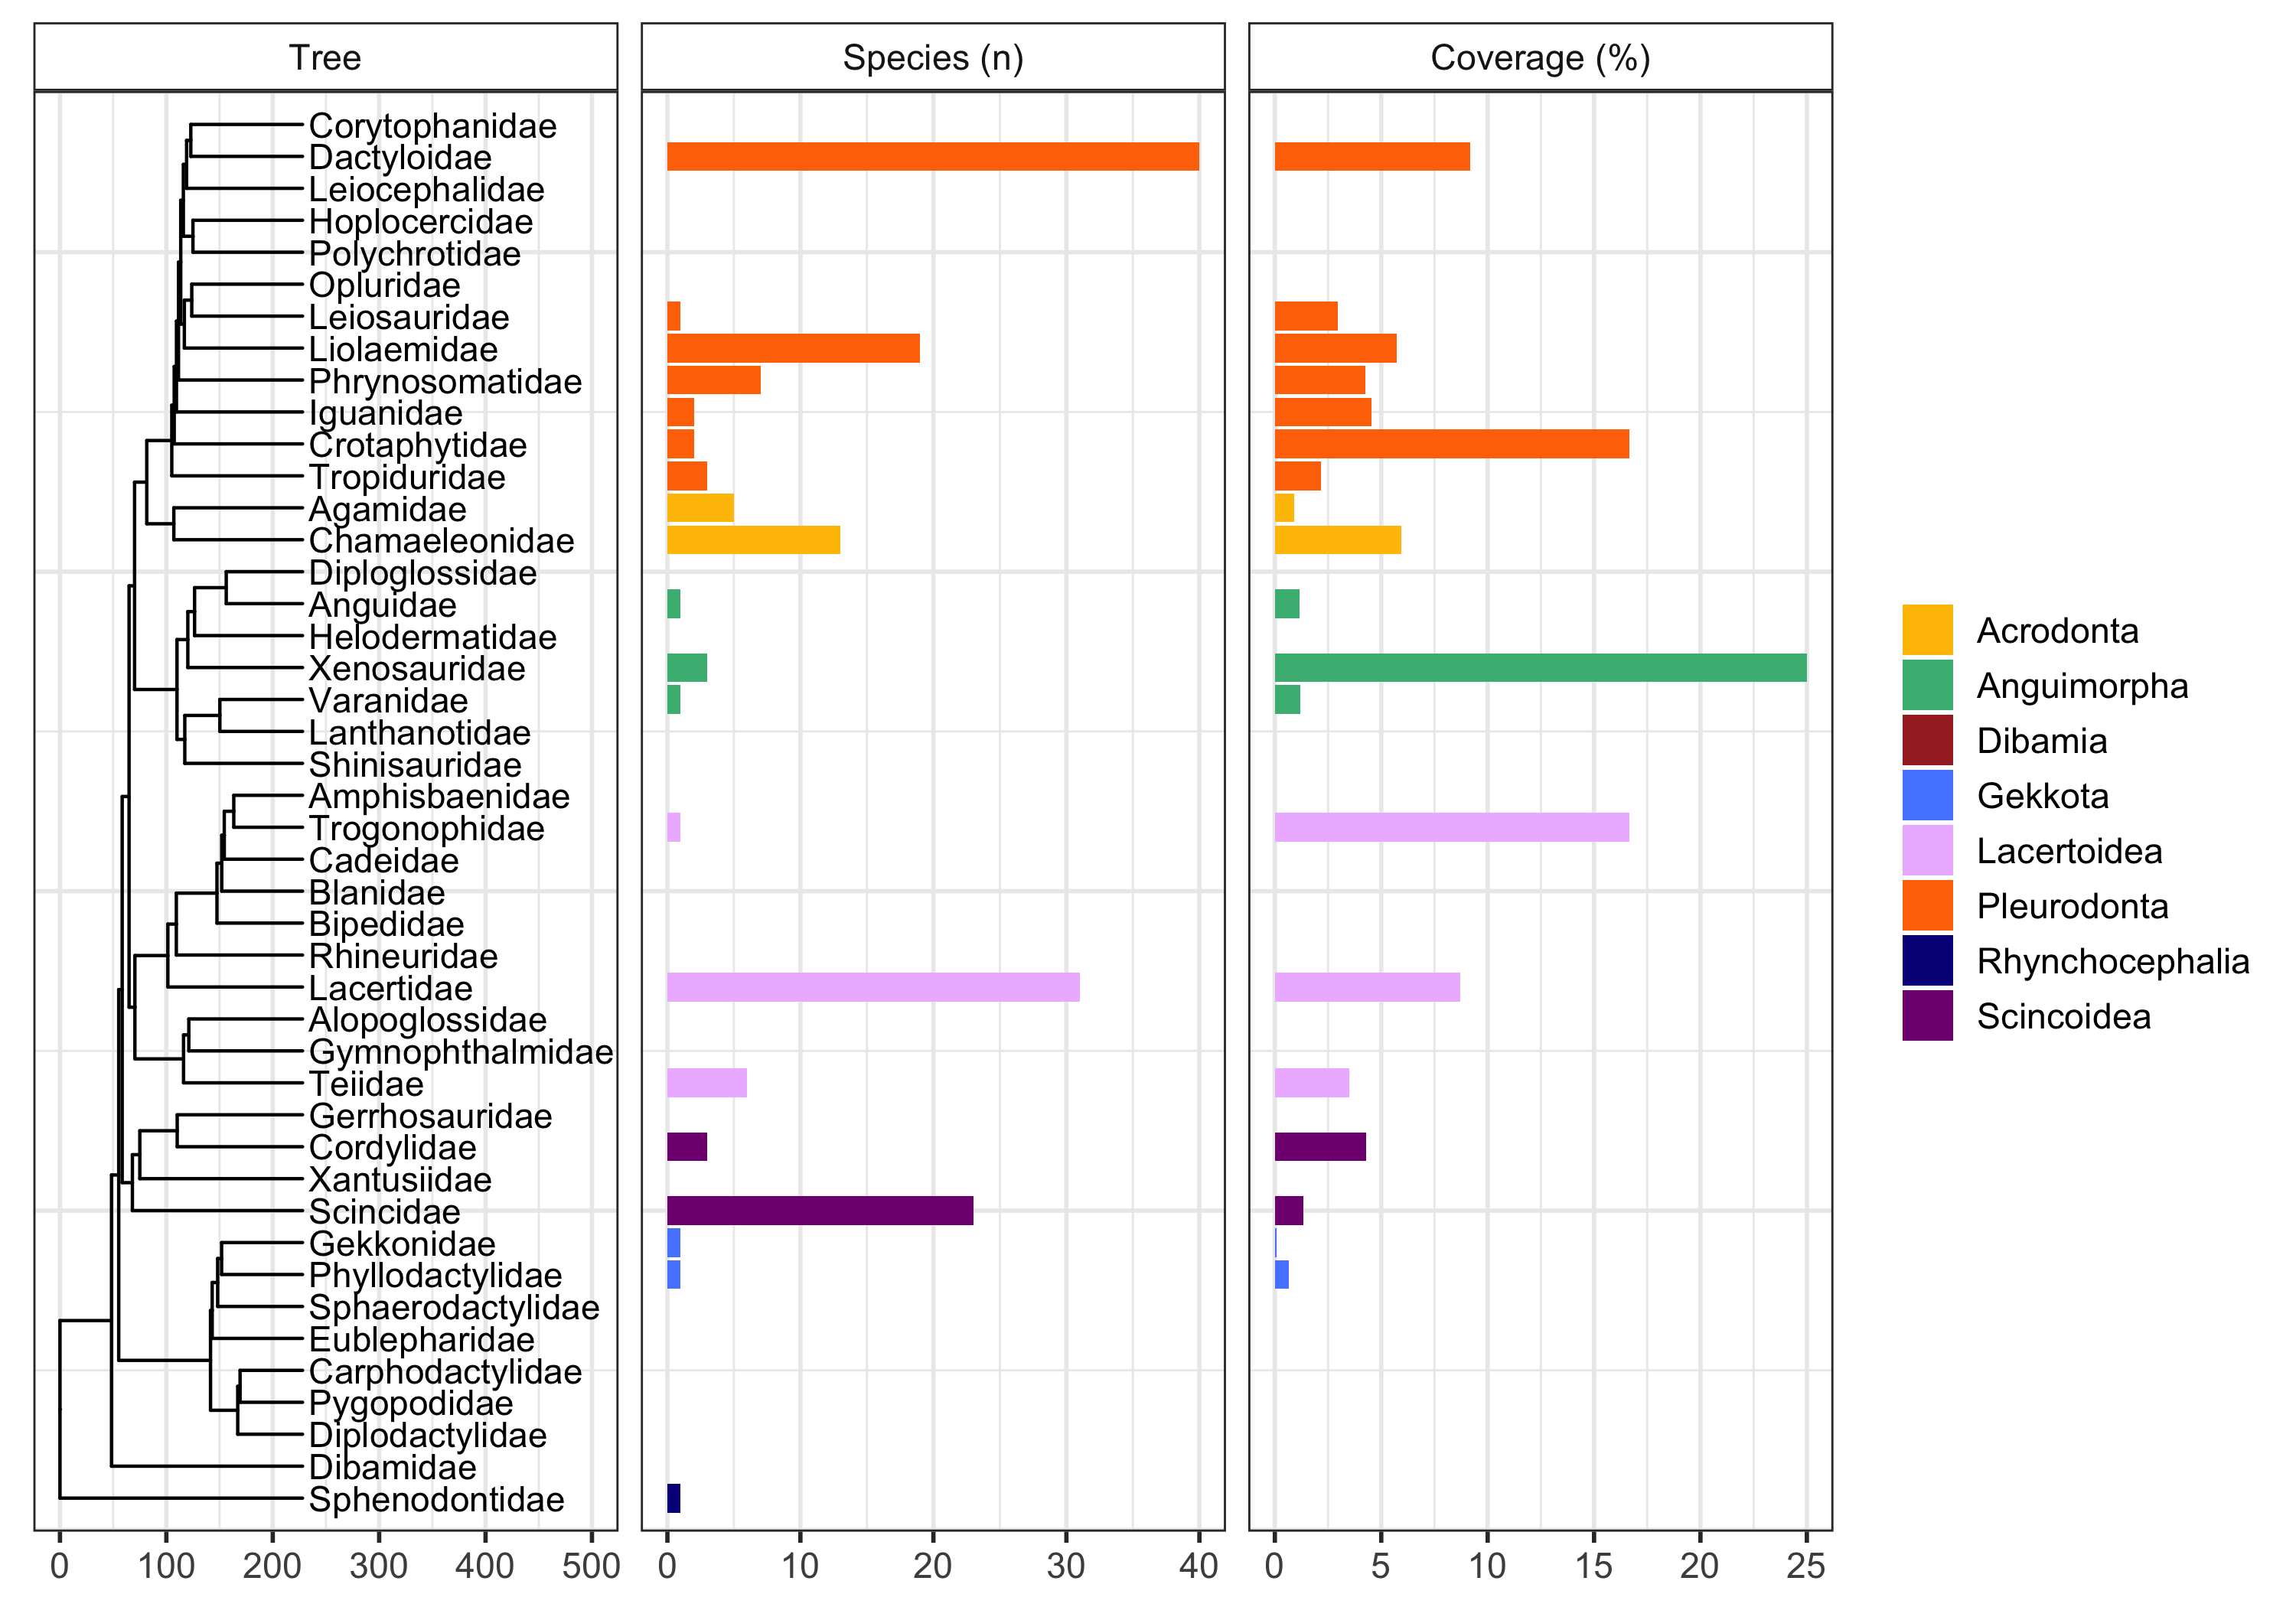
\includegraphics[width = \linewidth]{figures/phylogeny-data-coverage-colours.png}
  \caption{Family-level coverage of the bite-force dataset (n = 164 species). 
  The left-hand panel shows the family level phylogeny, the central panel shows the number of species from each family in our dataset, and the right-hand panel shows the percentage of species from that family from \cite{uetz2020reptile} that are in our dataset. 
  Sphenodontidae (Rhynchocephalia) contains only one species, \textit{Sphenodon punctatus}, and has 100\% coverage so was removed from the right-hand panel to prevent it from compressing the x-axis. 
  Colours indicate clades.
}
  \label{fig-data-coverage}
\end{figure}


% figure 2
\newpage
\begin{figure}[h]
 \centering
  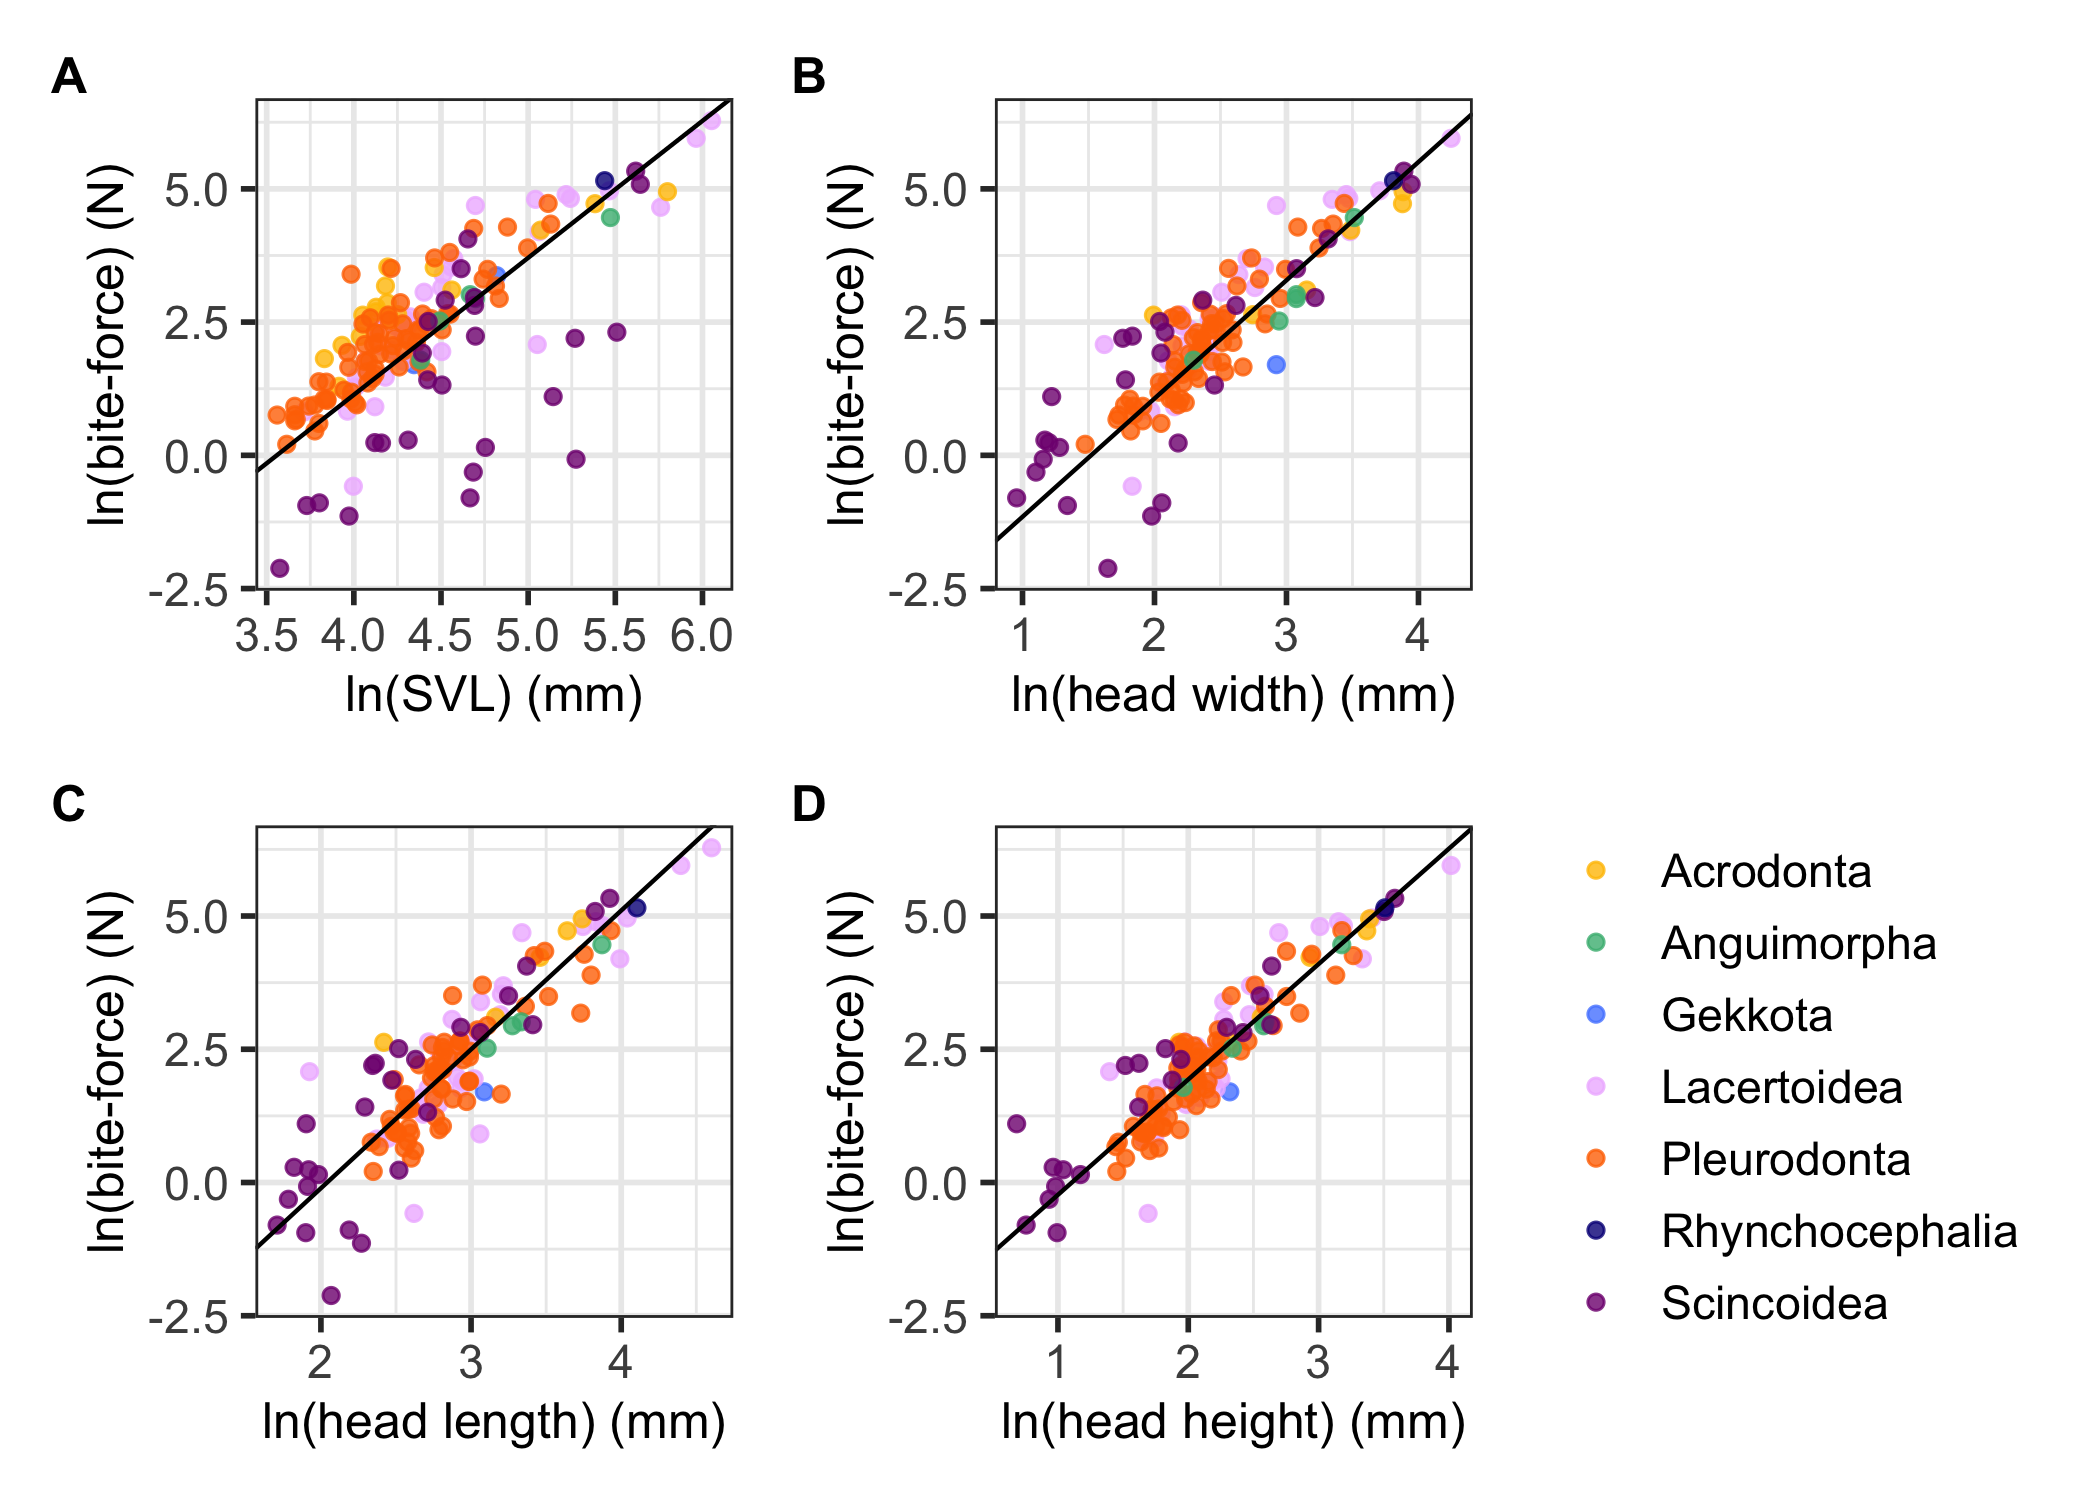
\includegraphics[width = \linewidth]{figures/bodysize-bite-force-coloured.png}
  \caption{The relationship between bite-force and each of the four size measures, with points coloured to identify clades. 
  (A) snout vent length (SVL; n = 161); (B) head width (n = 142); (C) head length (n = 136); and (D) head height (n = 136). 
  Points are slightly transparent to show where they overlap. 
  The lines are taken from phylogenetic generalised least squares (PGLS) models of bite-force as a function of size (Table S5). 
  There were no significant differences among clades (Table 1). 
  }
  \label{fig-size-biteforce}
\end{figure}


% figure 3
\newpage
\begin{figure}[h]
 \centering
  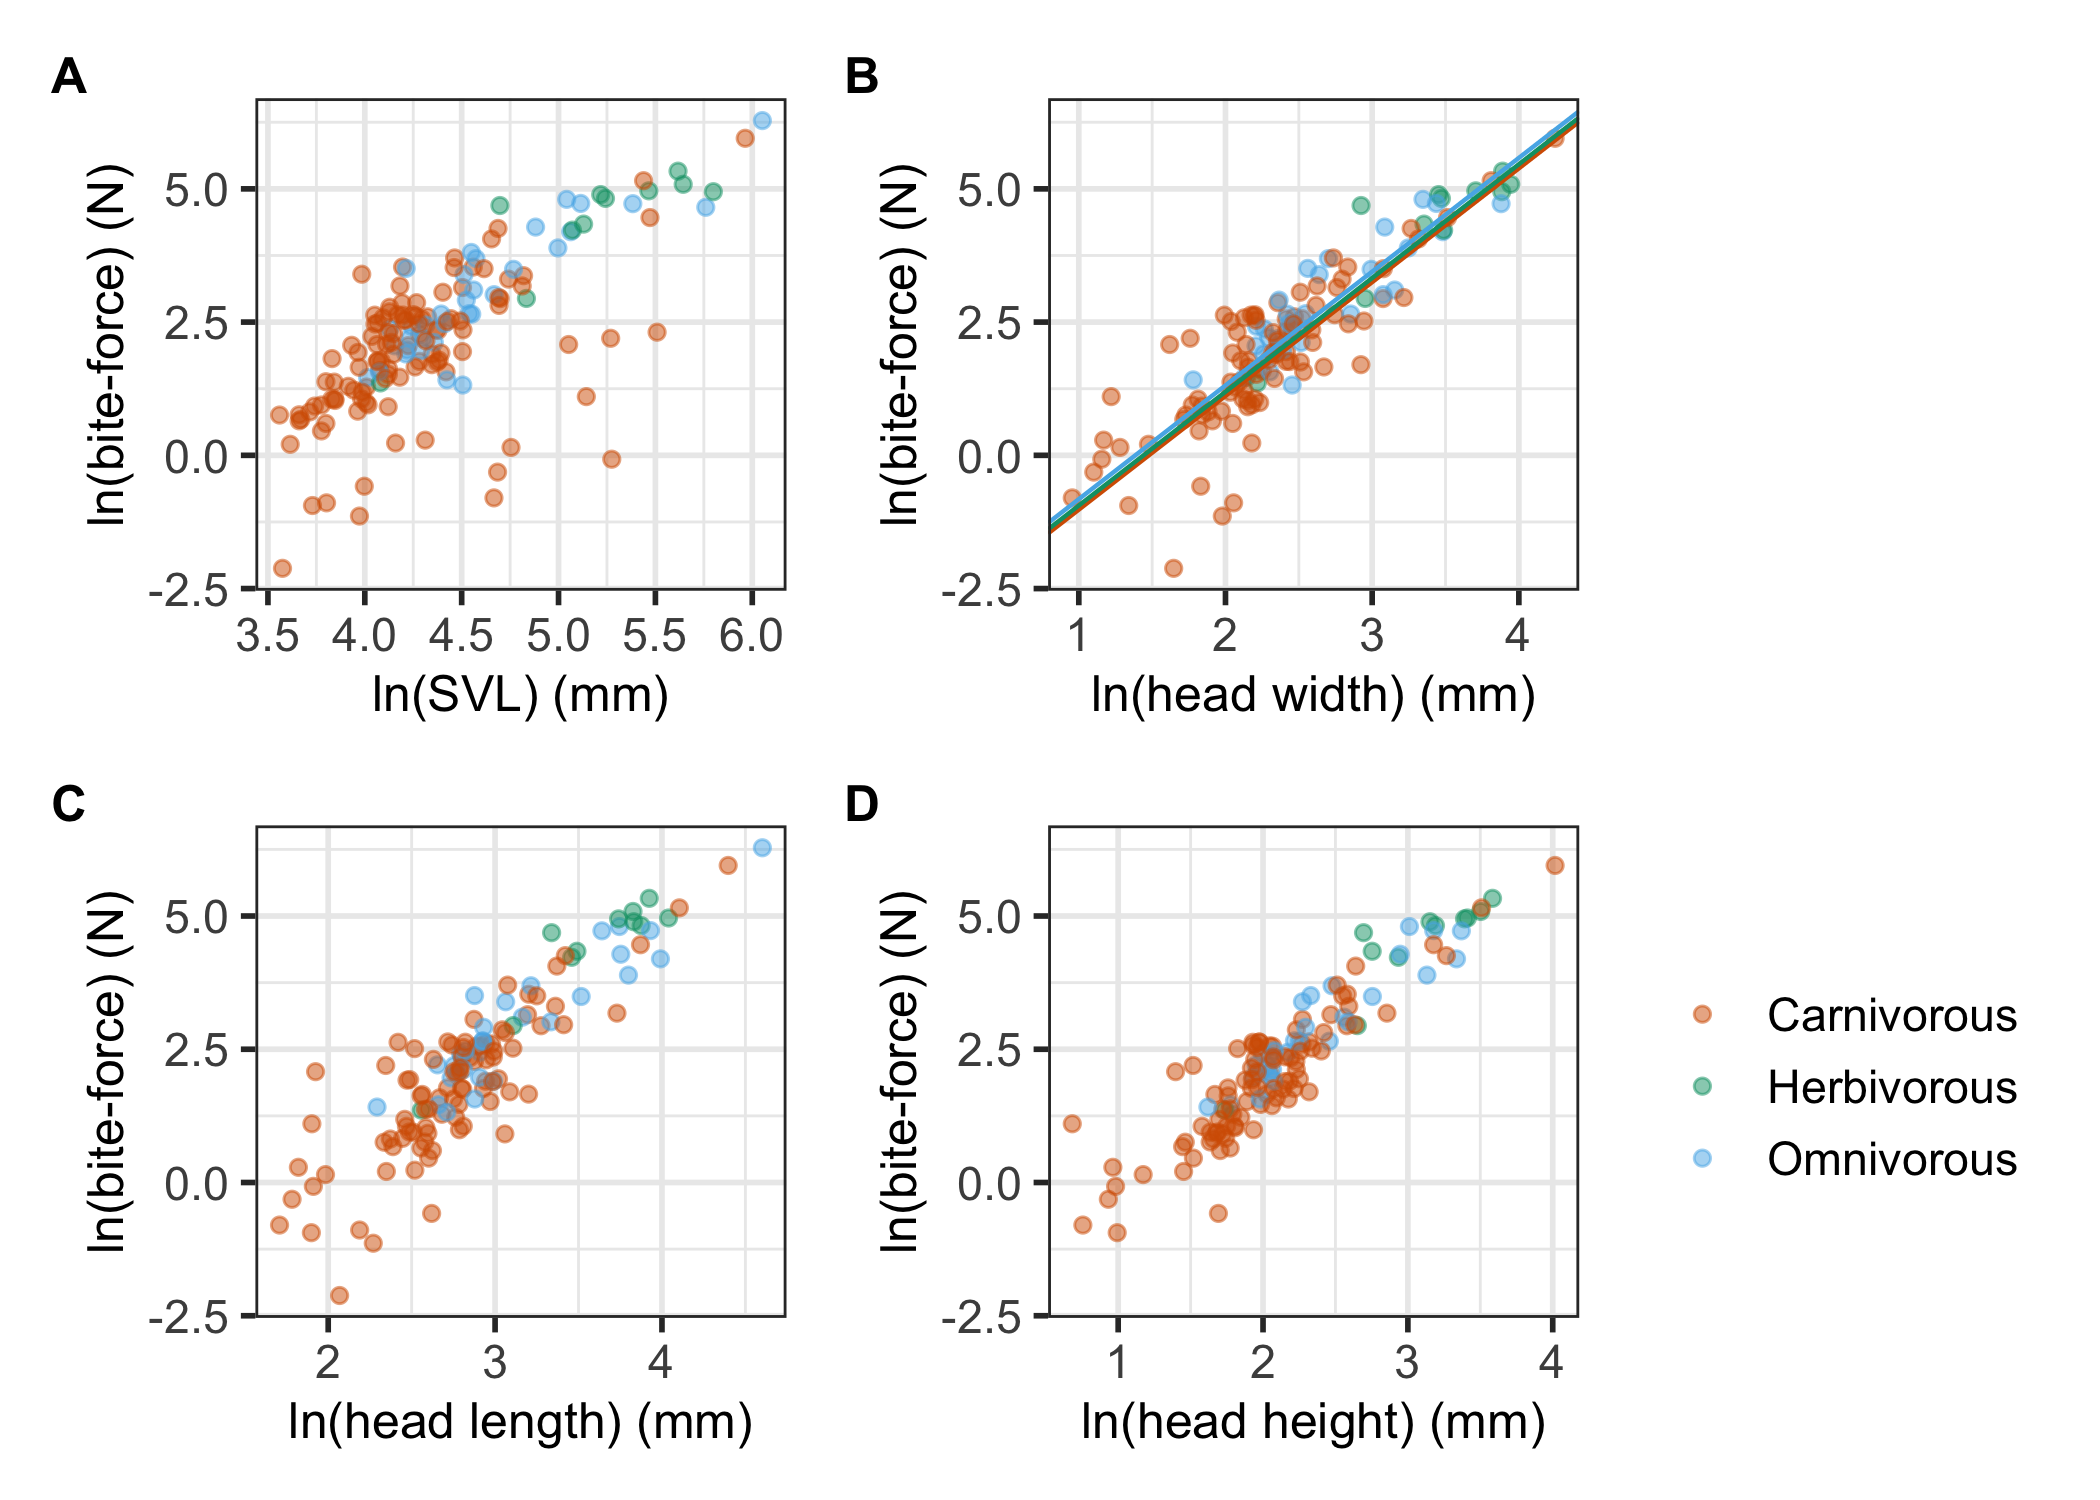
\includegraphics[width = \linewidth]{figures/bodysize-bite-force-diet.png}
  \caption{The relationship between bite-force and each of the four size measures for species with different diets. 
  (A) snout vent length (SVL; n = 158); (B) head width (n = 139); (C) head length (n = 133); and (D) head height (n = 133). 
  Points are slightly transparent to show where they overlap. 
  The lines in (B) are taken from a phylogenetic generalised least squares (PGLS) model of bite-force as a function of head width and diet, where different diets have significantly different intercepts (Table 1). 
  There were no significant differences among diets for the other three size measures (Table 1). 
}
  \label{fig-diet}
\end{figure}

% figure 4
\newpage
\begin{figure}[h]
 \centering
  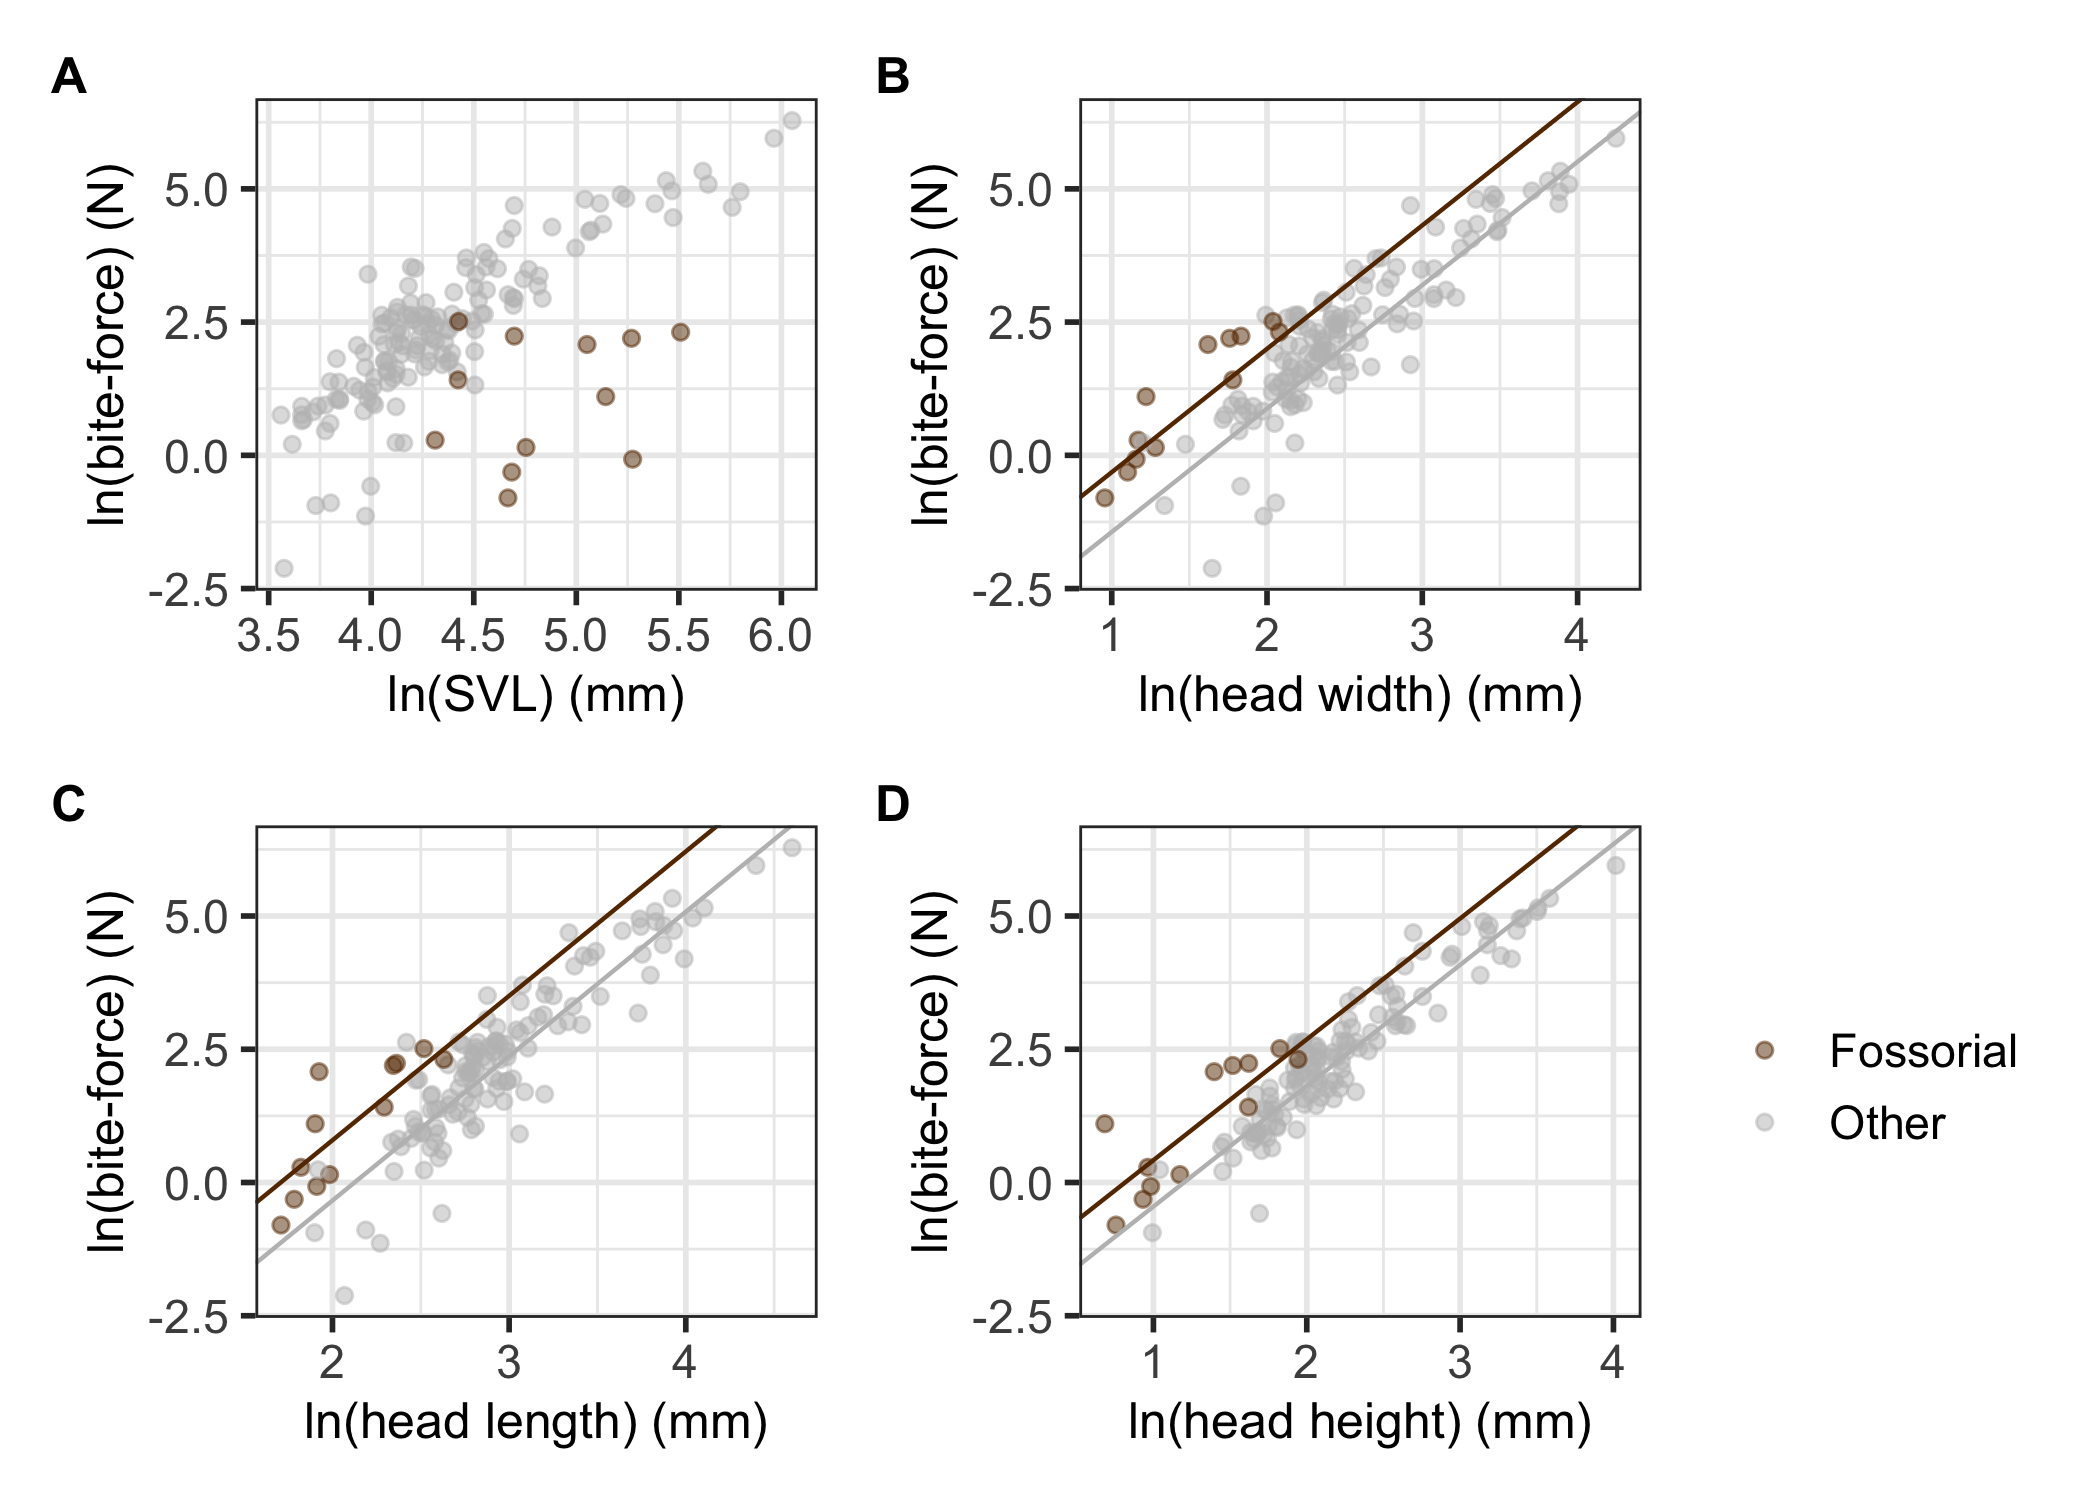
\includegraphics[width = \linewidth]{figures/bodysize-bite-force-fossorial.png}
  \caption{The relationship between bite-force and each of the four size measures for species that are purely fossorial and those that are not. 
  (A) snout vent length (SVL; n = 161); (B) head width (n = 142); (C) head length (n = 136); and (D) head height (n = 136). 
  Points are slightly transparent to show where they overlap. 
  The lines in (B-D) are taken from phylogenetic generalised least squares (PGLS) models of bite-force as a function of size and fossoriality, where fossorial and non-fossorial species have significantly different intercepts (Table 1). 
  There were no significant differences among fossorial and non-fossorial species for SVL (Table 1). 
}
  \label{fig-fossorial}
\end{figure}

\end{document}